\documentclass[tikz, border=2mm]{standalone}
\usepackage{amsmath}
\usepackage{fontspec}
\setmainfont{Times New Roman}
\usetikzlibrary{arrows.meta, positioning, shapes.geometric, calc}

\begin{document}
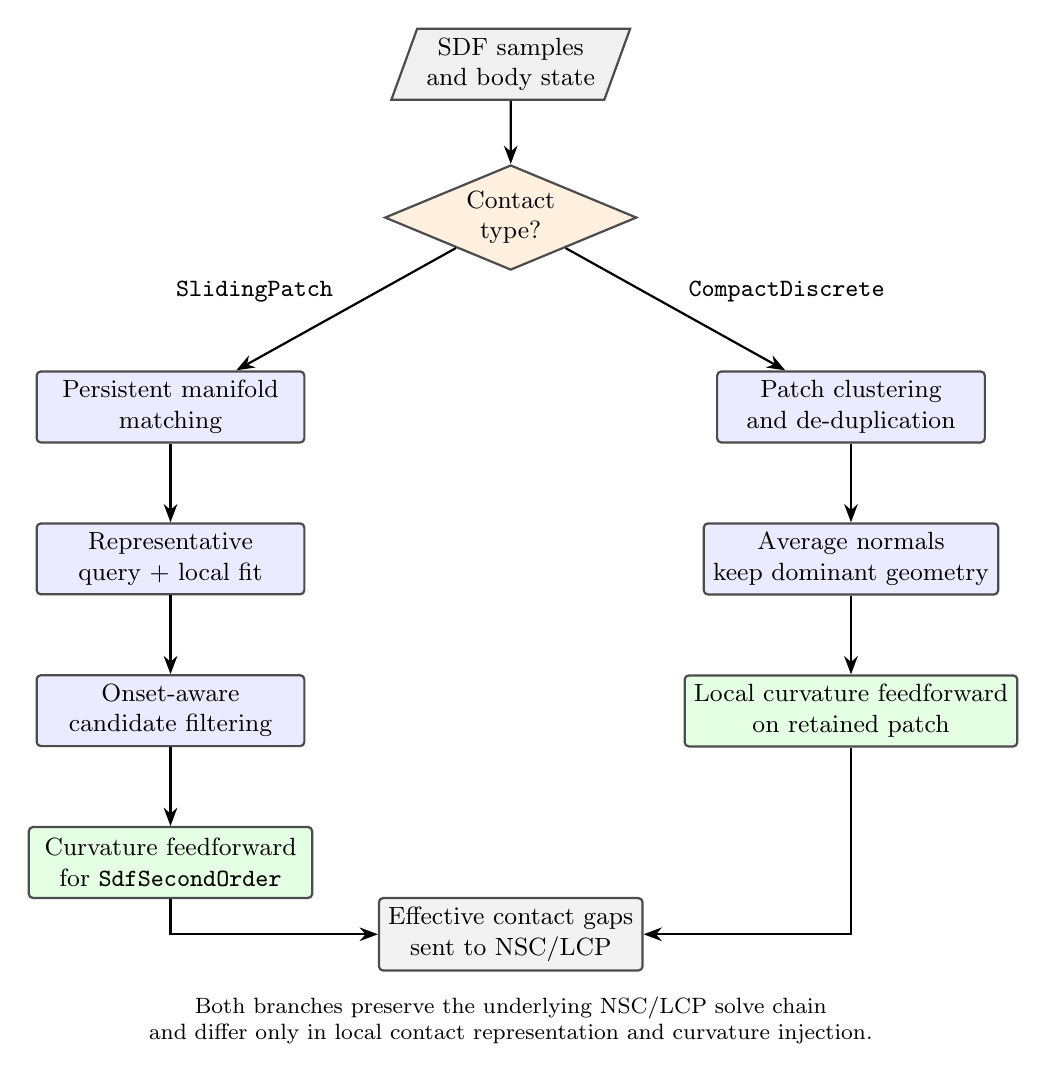
\begin{tikzpicture}[
    >=Stealth,
    node distance=10mm and 8mm,
    font=\small,
    io/.style={trapezium, trapezium left angle=70, trapezium right angle=110, draw=black!70, thick, fill=black!6, align=center, minimum width=30mm, minimum height=8mm},
    decision/.style={diamond, aspect=2.0, draw=black!70, thick, fill=orange!12, align=center, inner sep=1pt, minimum width=32mm, minimum height=10mm},
    proc/.style={rectangle, rounded corners=1.5pt, draw=black!70, thick, fill=blue!8, align=center, minimum width=34mm, minimum height=9mm},
    proc2/.style={rectangle, rounded corners=1.5pt, draw=black!70, thick, fill=green!10, align=center, minimum width=36mm, minimum height=9mm},
    outnode/.style={rectangle, rounded corners=1.5pt, draw=black!70, thick, fill=black!5, align=center, minimum width=30mm, minimum height=8mm},
    line/.style={->, thick}
]

\node[io] (input) {SDF samples\\and body state};
\node[decision, below=8mm of input] (regime) {Contact\\type?};

\node[proc, below left=16mm and 18mm of regime] (slide1) {Persistent manifold\\matching};
\node[proc, below=of slide1] (slide2) {Representative\\query + local fit};
\node[proc, below=of slide2] (slide3) {Onset-aware\\candidate filtering};
\node[proc2, below=of slide3] (slide4) {Curvature feedforward\\for \texttt{SdfSecondOrder}};

\node[proc, below right=16mm and 18mm of regime] (disc1) {Patch clustering\\and de-duplication};
\node[proc, below=of disc1] (disc2) {Average normals\\keep dominant geometry};
\node[proc2, below=of disc2] (disc3) {Local curvature feedforward\\on retained patch};

\coordinate (midpoint) at ($(slide4)!0.5!(disc3)$);
\node[outnode, below=14mm of midpoint] (output) {Effective contact gaps\\sent to NSC/LCP};

\draw[line] (input) -- (regime);
\draw[line] (regime) -- node[above left=-1pt and 1pt] {\texttt{SlidingPatch}} (slide1);
\draw[line] (regime) -- node[above right=-1pt and 1pt] {\texttt{CompactDiscrete}} (disc1);

\draw[line] (slide1) -- (slide2);
\draw[line] (slide2) -- (slide3);
\draw[line] (slide3) -- (slide4);
\draw[line] (disc1) -- (disc2);
\draw[line] (disc2) -- (disc3);

\draw[line] (slide4) |- (output);
\draw[line] (disc3) |- (output);

\node[below=2mm of output, align=center, font=\footnotesize] (note) {Both branches preserve the underlying NSC/LCP solve chain\\and differ only in local contact representation and curvature injection.};
\end{tikzpicture}
\end{document}
